\section{基本概念}
\begin{figure}[!htb]
    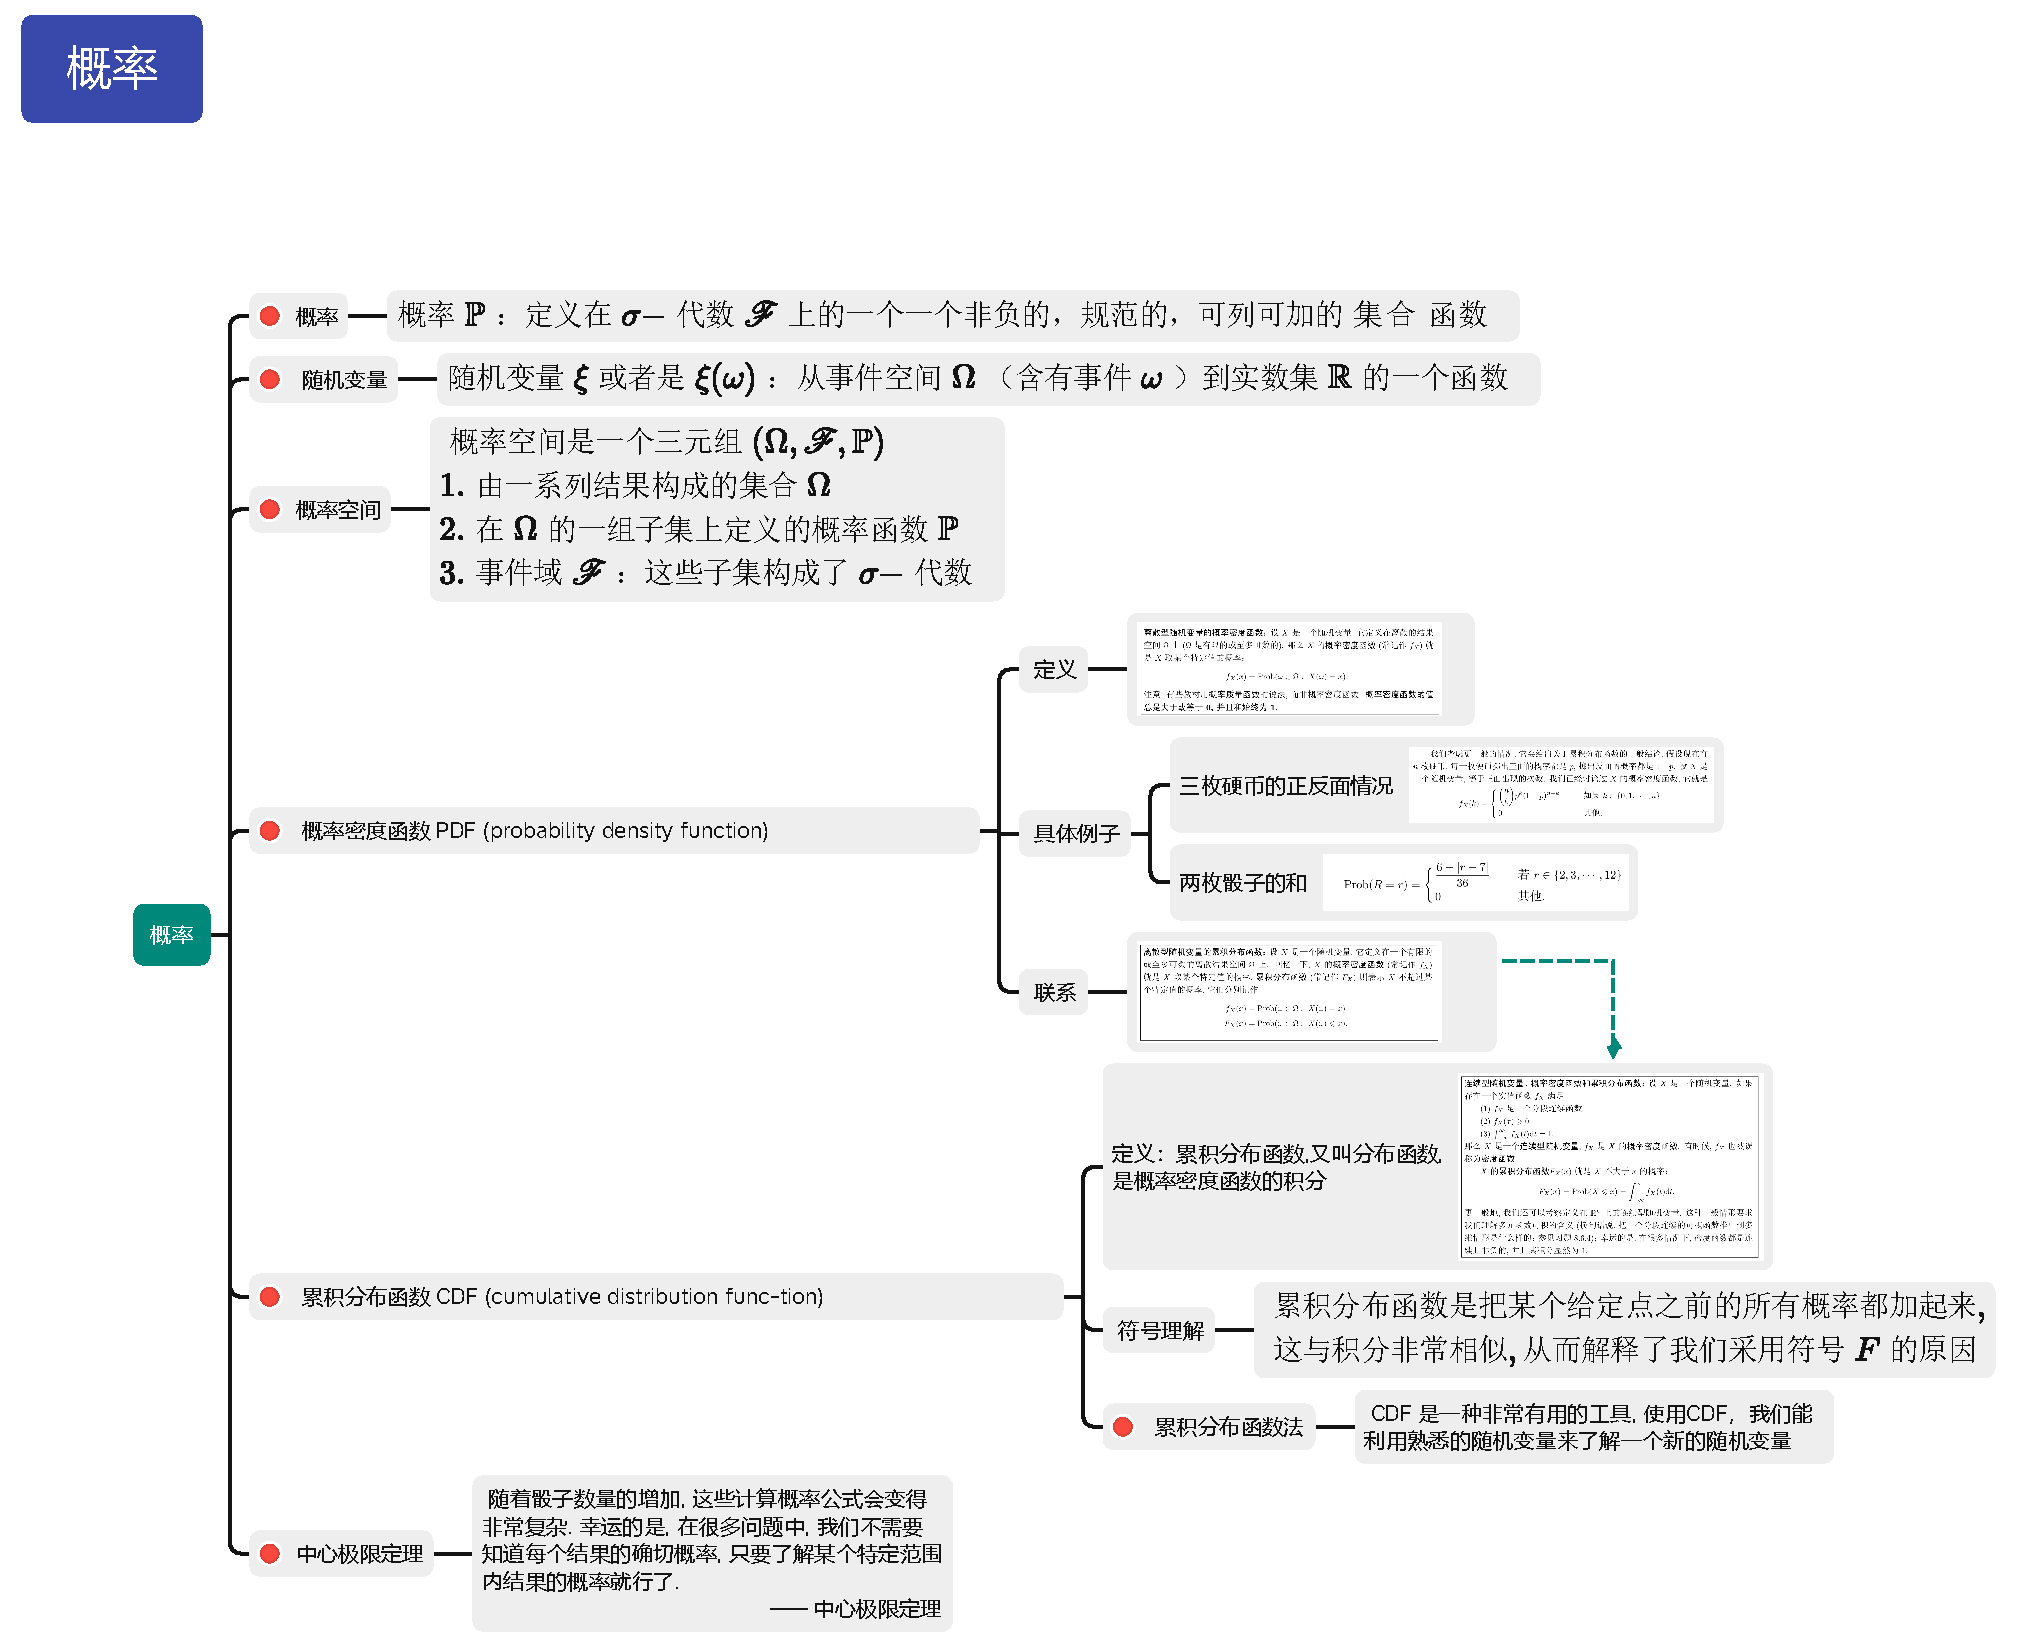
\includegraphics[scale=0.5]{Chapter/TikZ/概率.pdf}
    \label{概率基本对象}
    \caption{概率基本对象}
\end{figure}

\newpage
\section{常见的连续分布}

\begin{definition}[常见的连续分布]
    \num{1}\quad 均匀分布 \hspace*{4em} \num{2}\quad 指数分布
    \hspace*{4em}
    \num{3}\quad 正态分布 \hspace*{4em} \num{4}\quad $\beta$分布
\end{definition}


\noindent\num{1} {\sf 均匀分布}\par

\begin{align}
    \xi \sim \mathrm{U[a, b]}, ~~
    \mathrm{p(X)}=\begin{cases}
        \frac{1}{b-a},&a\le x\le b\\
        0, &\mathtext{其他}
    \end{cases}~~
    \mathrm{F(X)}=\begin{cases}
        0, & x<0\\
        \frac{x-a}{b-a}, &a\le x< b\\
        1,&x\ge b
    \end{cases}
\end{align}

\begin{center}
    \begin{tikzpicture}
        \draw[-stealth] (0, -1) -- (0, 2.5)node[right] {$\mathrm{p(X)}$};
        \draw[-stealth] (-1, 0) -- (6, 0)node[below] {$\mathrm{X}$};
        \node[black, left=8pt, below] at (0, 0) {$O$};
        \draw[red] (-0.3, 0) -- (1, 0);
        \draw[dashed] (1, 1) -- (0, 1);
        \draw[red] (1, 1) -- (2, 1);
        \draw[red] (2, 0) -- (5, 0);
        \node[below, red] at (2, 0) {$b$};
        \node[below, red] at (1, 0) {$a$};
        \draw[dashed, red] (1, 0) -- (1, 1);
        \draw[dashed, red] (2, 0) -- (2, 1);
        \node[left] at (0, 1) {$\frac{1}{b-a}$};
        \draw[fill=black] (0, 1) circle [radius=1pt];
        \draw[draw=black] (1, 0) circle [radius=1pt];
        \draw[draw=black] (2, 0) circle [radius=1pt];
        \node at (3.5, -1) {\mathtext{显然,}$\mathrm{p(X)}$\mathtext{在}$\mathrm{X=a, X=b}$\mathtext{处均不连续。}}; 
    \end{tikzpicture}  
    \begin{tikzpicture}
        \draw[-stealth] (0, -1) -- (0, 2.5)node[right] {$\mathrm{F(X)}$};
        \draw[-stealth] (-1, 0) -- (6, 0)node[below] {$\mathrm{X}$};
        \node[black, left=8pt, below] at (0, 0) {$O$};
        \draw[red] (-0.3, 0) -- (1, 0)node[below] {$a$} -- (2, 1) -- (5, 1);
        \node[below, red] at (2, 0) {$b$};
        \draw[dashed] (2, 0) -- (2, 1) -- (0, 1);
        \node[left] at (0, 1) {$\mathrm{1}$};
        \draw[fill=black] (0, 1) circle [radius=1pt];
        \draw[fill=black] (1, 0) circle [radius=1pt];
        \draw[fill=black] (2, 0) circle [radius=1pt];
        \node at (3.5, -1) {\mathtext{显然,}$\mathrm{F(X)}$\mathtext{在所有点处均连续。}}; 
    \end{tikzpicture}      
\end{center}


\noindent\num{2} {\sf 指数分布}\par
\begin{align}
    \mathtext{记作}\xi \sim \mathrm{Exp}(\lambda),~~p(x)=\begin{cases}
    \lambda e^{-\lambda x},&x>0\\
    0,~~~&x\le0
    \end{cases}~~
    F(x) = \begin{cases}
    1-e^{-\lambda x},~~~x>0\\
    0,~~~x\le0
    \end{cases}
\end{align}

\begin{center}
    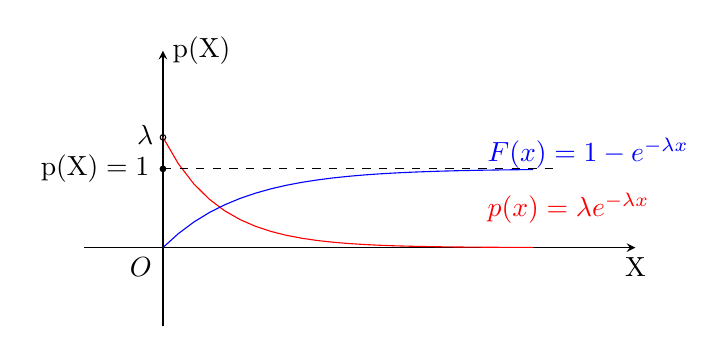
\begin{tikzpicture}
        \draw[-stealth] (0, -1) -- (0, 2.5)node[right] {$\mathrm{p(X)}$};
        \draw[-stealth] (-1, 0) -- (6, 0)node[below] {$\mathrm{X}$};
        \node[black, left=8pt, below] at (0, 0) {$O$};
        \draw[domain=0:4.7, red] plot(\x, {1.4*exp(-1.4*\x)});
        \node[right, red] at (4, 0.5) {$p(x)=\lambda e^{-\lambda x}$};
        \node[left] at (0, 1.43) {$\lambda$};
        \draw (0, 1.4) circle [radius=1pt];
        \draw[domain=0:4.7, blue] plot(\x, {1-exp(-\x)});
        \draw[dashed] (0, 1)node[left, circle, radius=1pt] {$\mathrm{p(X)=1}$} -- (5, 1);
        \draw[fill=black] (0, 1) circle [radius=1pt];
        \node[right, blue] at (4, 1.2) {$F(x)=1- e^{-\lambda x}$};
    \end{tikzpicture}        
\end{center}



设随机变量具有密度函数
\begin{align}
    \Rm{p(x)}=\frac{1}{\sqrt{2\pi}\sigma}\Rm{e}^{-\frac{(x-\mu)^2}{2\sigma^2}},  ~~~-\infty<\rm{x}<+\infty
\end{align}

其中$\mu, \sigma$ 为常数,则称$\xi$服从参数为$\mu, \sigma$的正态分布或Gauss分布,记作$\xi \sim N(\mu, \sigma^2)$.其分布函数为:
\begin{align}
    F(x)=p(\xi \le x)=\int_{-\infty}^{x}{p(y) \dd y}=\frac{1}{\sqrt{2\pi}\sigma} \int_{-\infty}^{x}{\Rm{e}^{-\frac{(y-\mu)^2}{2\sigma^2}} \dd y} , ~~~ -\infty<x<+\infty
\end{align}

\begin{center}
    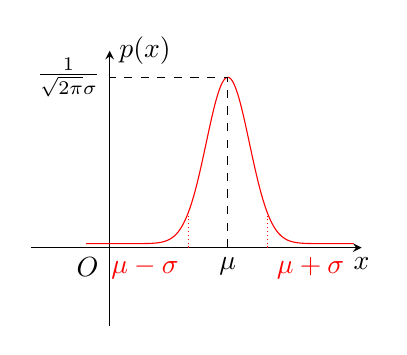
\begin{tikzpicture}
        \draw[-stealth] (0, -1) -- (0, 2.5)node[right] {${p(x)}$};
        \draw[-stealth] (-1, 0) -- (3.2, 0)node[below] {${x}$};
        \node[black, left=8pt, below] at (0, 0) {$O$};
        \draw[domain=-0.3:3.1, red, samples=1000] plot(\x, {1/(sqrt(2*pi))*exp(-(\x-1)*(\x-2)/(0.15))+0.05});
        \draw[dashed] (1.5, 0)node[below] {$\mu$} -- (1.5, 2.16) -- (0, 2.16)node[left] {$\frac{1}{\sqrt{2\pi}\sigma}$};
        \draw[densely dotted, red] (1, 0)node[below left] {$\mu-\sigma$} -- (1, 0.4);
        \draw[densely dotted, red] (2, 0)node[below right] {$\mu+\sigma$} -- (2, 0.4);
    \end{tikzpicture}        
\end{center}



\section{ARMA模型}
\begin{figure}[!htb]
    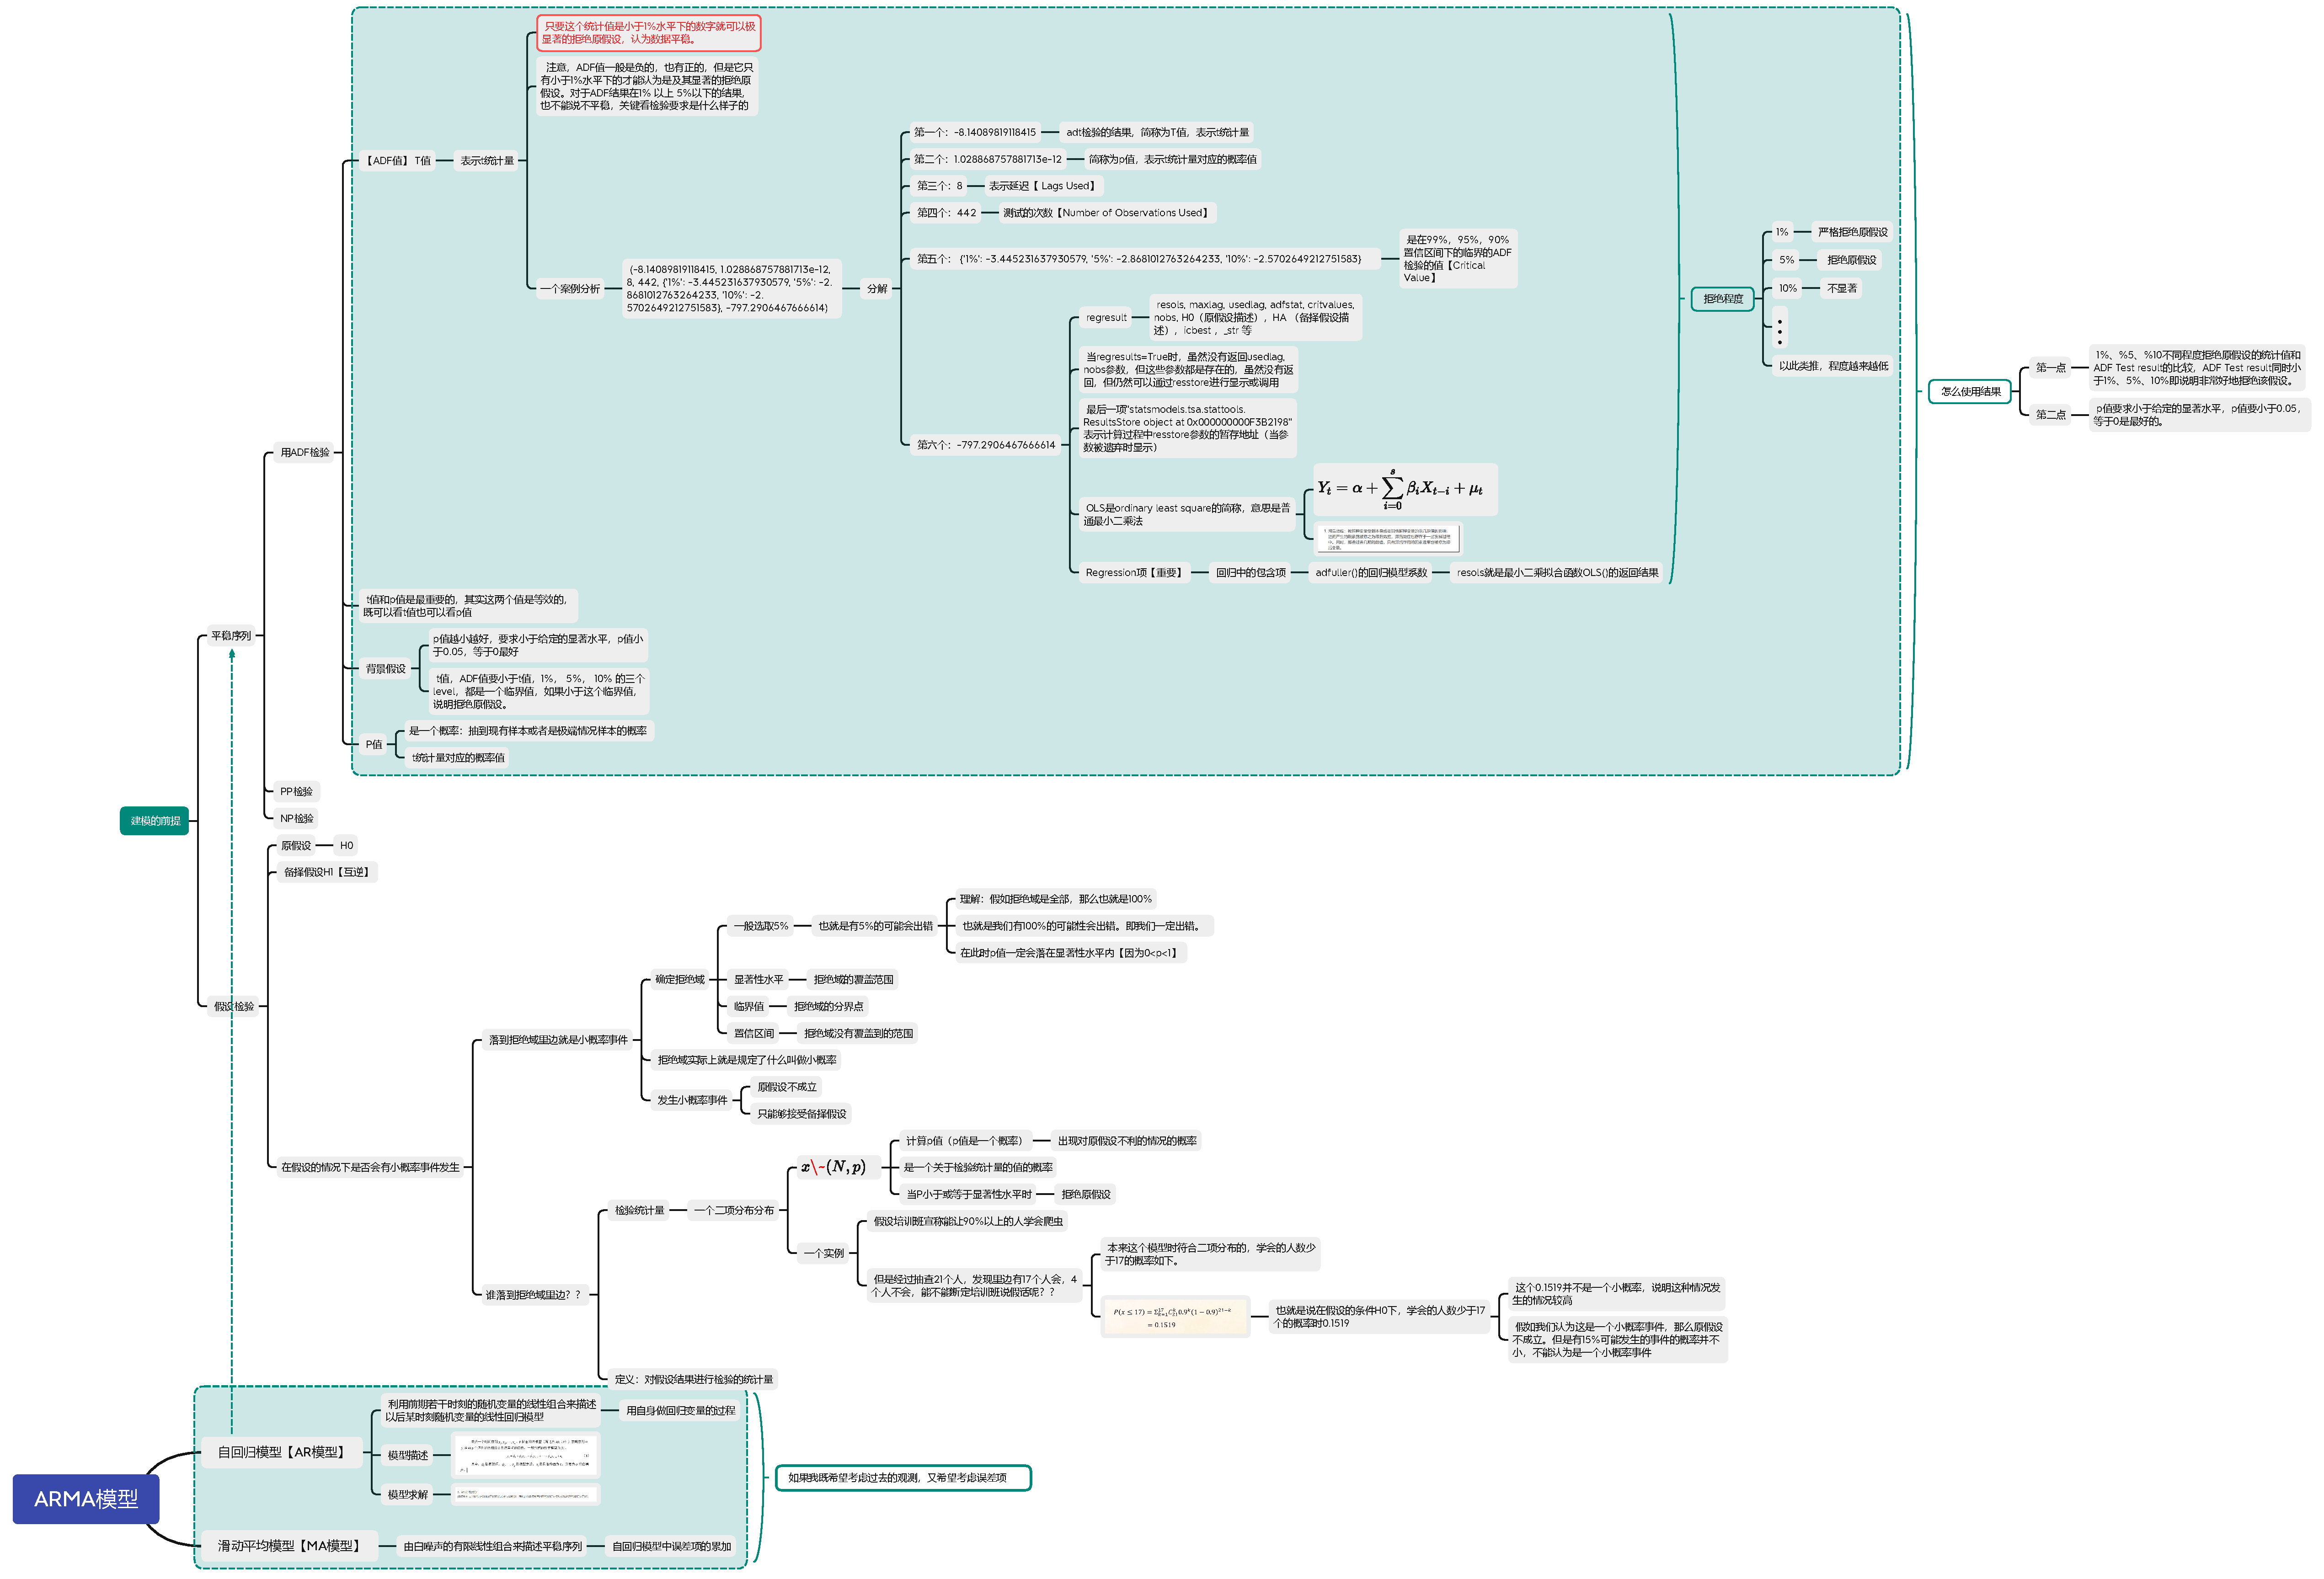
\includegraphics[scale=0.2]{Chapter/TikZ/ARMA模型.pdf}
    \label{ARMA模型}
    \caption{ARMA模型}
\end{figure}